\documentclass[10pt,a4paper,openany]{beamer}
\usepackage[utf8]{vietnam}
\usepackage{lmodern}
\usetheme{AnnArbor}
\usecolortheme{beaver}
\usepackage{tikz}
\usepackage{smartdiagram}

\AtBeginSection[]
{
	\begin{frame}<beamer>
		\frametitle{Nội dung}
		\tableofcontents[currentsection]
		
		\raggedright\tiny\textsuperscript{} Source code: https://gitlab.com/fakerphan/masr2
		
		\raggedright\tiny\textsuperscript{} Documents: https://gitlab.com/fakerphan/masr2/tree/master/reports
	\end{frame}
}

\author[Phan Xuan Phuc]{
\includegraphics[scale=0.1]{charts/logo.png}\\Phan Xuan Phuc\\Mentor: TS. Nguyen Hong Quang}
\title{Thử nghiệm nhận dạng tiếng nói tiếng Việt cho người khuyết tật giọng nói bằng phương pháp học sâu}
\institute[HUST]{Hanoi University of Science and Technology\\}
\date{Ha Noi, January 14, 2020}
%
%
\newcommand{\argmax}{\arg\!\max}
%\subject{}
\tikzstyle{startstop} = [rectangle, rounded corners, minimum width=1.5cm, minimum height=0.6cm,text centered, draw=black, fill=red!30]
\tikzstyle{process} = [rectangle, minimum width=1.5cm, minimum height=0.6cm, text centered, draw=black, text width=2cm, fill=orange!30]
\tikzstyle{arrow} = [thick,->,>=stealth]

\setbeamertemplate{caption}[numbered] 
\begin{document}
	\listoffigures

	\begin{frame}
		\titlepage
	\end{frame}

	\begin{frame}
		\frametitle{Nội dung}
		\tableofcontents
		
		\raggedright\tiny\textsuperscript{} Source code: https://gitlab.com/fakerphan/masr2
		
		\raggedright\tiny\textsuperscript{} Documents: https://gitlab.com/fakerphan/masr2/tree/master/reports
	\end{frame}
	
	
	\section{Giới thiệu bài toán}
	\begin{frame}{Giới thiệu bài toán}
		\emph{Với những người bị khuyết tật giọng nói, làm sao để mọi người có thể hiểu những gì họ nói?} \pause
		\begin{columns}
		\begin{column}{0.6\textwidth}						
		\begin{itemize}
			\item{Nhận dạng tiếng nói của người bị khuyết tật giọng nói\\}
			$\rightarrow$ "Speech Recognition" \pause
			\begin{itemize}
				\item{Biến đổi tiếng nói (Speech) $\rightarrow$ văn bản (Text)}
			\end{itemize}							
		\end{itemize}
		\end{column}
		\begin{column}{0.4\textwidth}
		\begin{figure}[htbp]
		\centerline{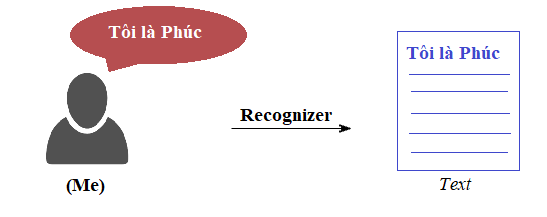
\includegraphics[scale=0.35]{charts/intro.png}}
		\label{fig_intro}
		\end{figure}	 \pause
		\end{column}
		\end{columns}
		\begin{itemize}
			\item{Tập trung vào tiếng nói của người bị khuyết tật giọng nói}  \pause
			\item{Tập trung với ngôn ngữ Tiếng Việt} \pause
		\end{itemize}
		\textbf{Input:} Một âm thanh tiếng nói (Speech) của người khuyết tật giọng nói \\ \pause
		\textbf{Output:} Văn bản đầu ra (Text) tương ứng của âm thanh tiếng nói đó\pause
	\end{frame}
	
	\begin{frame}{Motivation}
		\begin{columns}
			\begin{column}{0.5\textwidth}
				\begin{figure}[htbp]
					\centerline{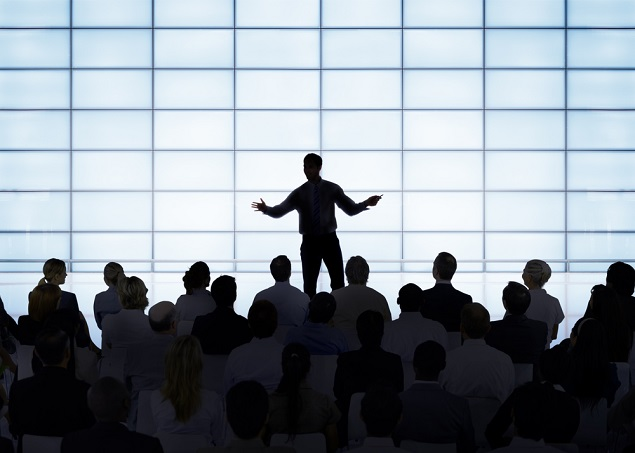
\includegraphics[scale=0.8]{charts/motivation.jpg}}
					\label{fig_motivation1} \pause
				\end{figure} 
				\begin{figure}[htbp]
					\centerline{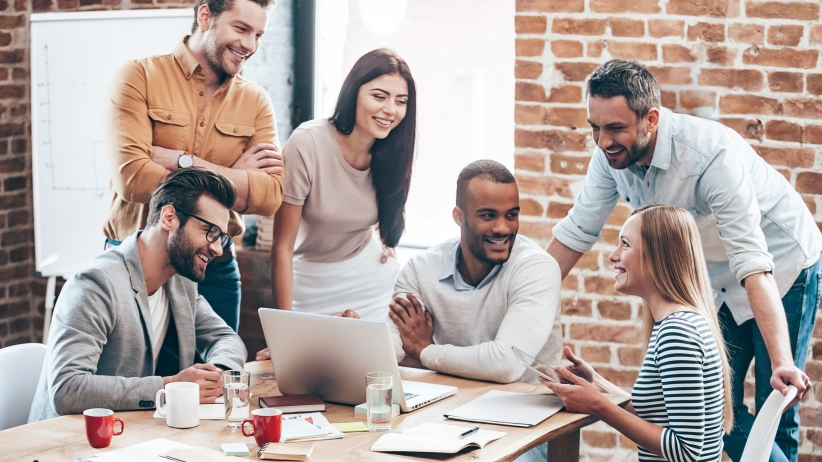
\includegraphics[scale=0.15]{charts/motivation2.jpg}}
					\label{fig_motivation2} \pause
				\end{figure} 
			\end{column}
			\begin{column}{0.5\textwidth}
				\begin{figure}[htbp]
					\centerline{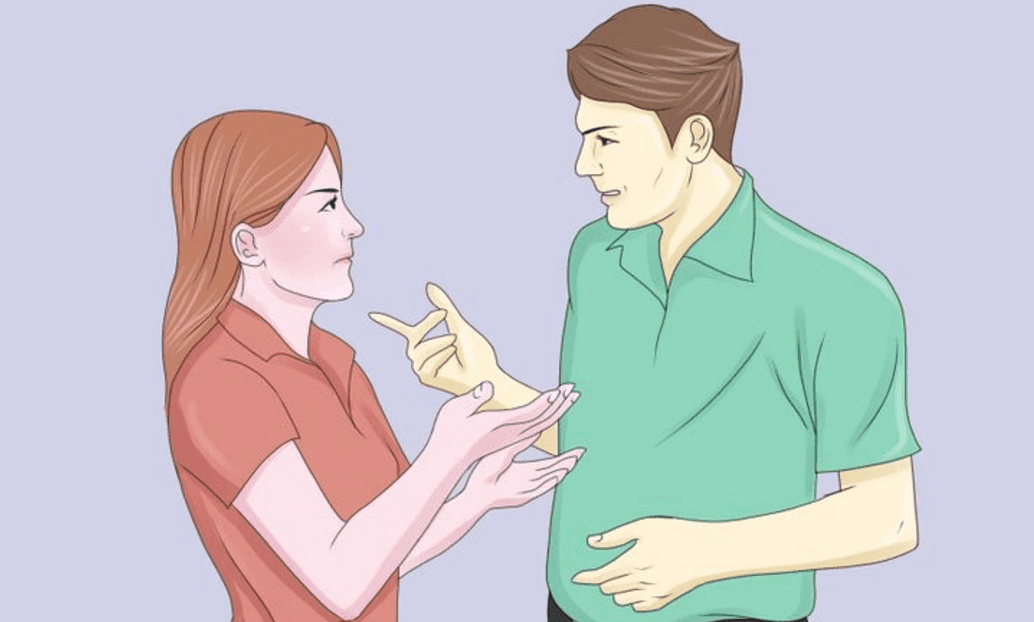
\includegraphics[scale=0.15]{charts/motivation4.png}}
					\label{fig_motivation3}
				\end{figure}
				\begin{figure}[htbp]
					\centerline{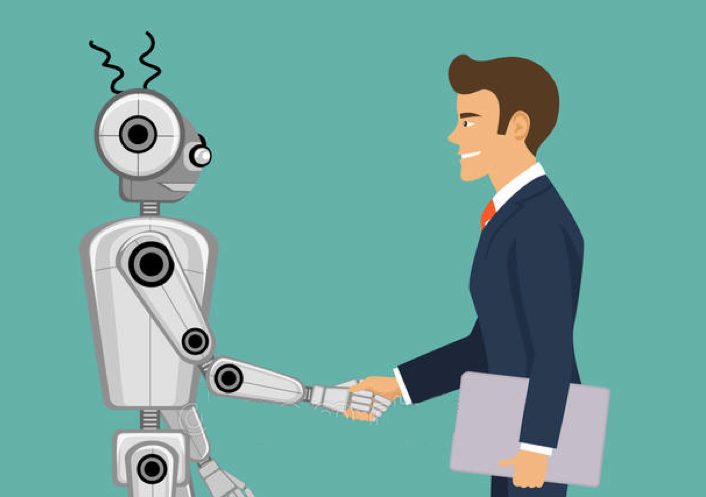
\includegraphics[scale=0.22]{charts/motivation3.png}}
					\label{fig_motivation4}
				\end{figure}
			\end{column}
		\end{columns}
	\end{frame}

	\section{Dataset}
	\def\MyScale{.2}
	\def\MySpace{0cm}
	\begin{frame}{Dataset}
		\textbf{Ngữ cảnh:} \\  \pause
		\begin{itemize}
			\item Chỉ có khoảng 3 tháng để thực hiện \pause
			\item Không có dữ liệu có sẵn của người khuyết tật giọng nói \pause
		\end{itemize}
		\textbf{Giải pháp:} \pause
		\begin{itemize}
			\item Thu thập dữ liệu bằng cách ghi âm 1600 từ vựng thông dụng nhất trong Tiếng Việt \footnote{ Wiki, \text{\color{blue} https://www.ezglot.com/most-frequently-used-words.php?l=vie\&s=wp-freq.}} sao cho bao phủ toàn bộ âm vị và chữ cái trong Tiếng Việt, \pause
			\begin{itemize}
				\item Bao gồm: 134 âm vị, 89 chữ cái (bao gồm cả thanh điệu),  \pause
				\item Bao gồm: 1546 từ đơn, 54 từ ghép, \pause
			\end{itemize}			
			\item Có 3 người nói (speaker): \pause
			\begin{itemize}
				\item 3 Man (Bố, Anh Trai và Tôi),
				\item 0 Woman,\pause
			\end{itemize} 
			\item Mỗi từ vựng được ghi âm bởi 3 người và ở 4 thời điểm nói khác nhau, \pause
			\item Training: 3*(1,600 ghi âm/ 1 người) ở 3 thời điểm nói, \pause
			\item Evaluation: 3*(1,600 ghi âm/ 1 người) ở thời điểm nói còn lại.
		\end{itemize}
	\end{frame}
	
	\begin{frame}{Dataset}
		\begin{figure}[htbp]
			%\vspace{\MySpace}
			\centerline{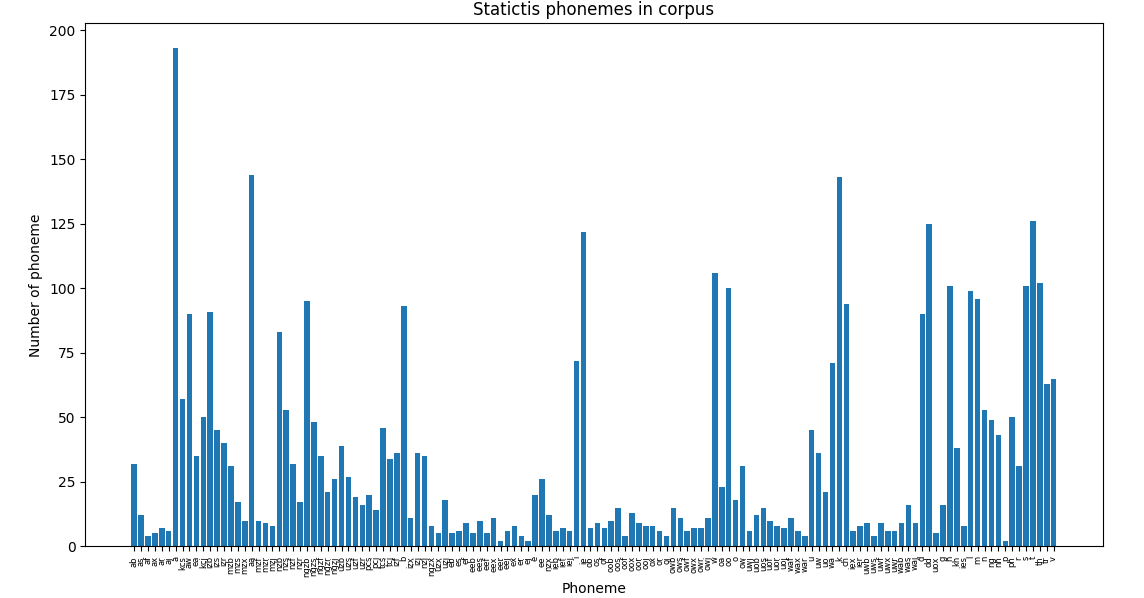
\includegraphics[scale=0.25]{charts/distribution_phonemes.png}}
			\caption{Phân bố 134 âm vị tiếng Việt trong bộ dữ liệu thu thập gồm 1,600 từ vựng \emph{\color{red}$\rightarrow$ Mất cân bằng (Imbalacing)}}
			\label{fig_distribution_phonemes}
		\end{figure}
	\end{frame}
	
	\section{Định hướng giải pháp}
	\begin{frame}{Định hướng giải pháp}
		\begin{center}
			\smartdiagramanimated[priority descriptive diagram]{
				Xử lý dữ liệu,
				Thực hiện trích xuất đặc trưng,
				Xây dựng mô hình âm học (Acoustic Model),
				Decoding}
		\end{center}
	\end{frame}
	
	\section{Giải quyết bài toán}
	\begin{frame}{Xử lý dữ liệu}
		\begin{itemize}
			\item Dữ liệu thu âm được lưu trữ dưới định dạng .mp3 hoặc .m4a \pause
			\item Chuyển đổi dữ liệu âm thanh thành định dạng .wav, mono-chanel, sampling rate=16kHz: \pause
			\begin{block}{Command line (Linux):}
				for f in *.m4a; do ffmpeg -i "\$f" -acodec pcm\_s16le -ac 1 -ar 16000 "\${f/\%m4a/wav}"; done \pause
			\end{block}
			\item Sử dụng thư viện Librosa \footnote{\text{\color{blue}https://librosa.github.io/librosa/}} để thực hiện đọc file âm thanh từ file .wav
		\end{itemize}
	\end{frame}
	
	\begin{frame}{Xử lý dữ liệu}
		\begin{block}{Cân bằng dữ liệu tập huấn luyện} \pause
			\begin{itemize}
				\item Ta xét một ngưỡng cân bằng N (N=100) \pause
				\item Với những âm vị có số lần xuất hiện < N $\rightarrow$ Cluster A, \\ngược lại $\rightarrow$ Cluster B \pause
				\item Với những âm vị trong Cluster A, ta thực hiện việc tăng cường số lần xuất hiện của nó bằng cách:  \pause
				\begin{itemize}
					\item Tìm kiếm từ (word) tương ứng có chứa âm vị đó, sao cho: Các âm vị được phân tích bởi từ đó có nhiều nhất có thể trong Cluster A và ít tồn tại nhất có thể trong Cluster B \pause
				\end{itemize}
				\item Thuật toán dừng lại cho đến khi tất cả các âm vị vượt qua ngưỡng cân bằng $\rightarrow$ Bộ dữ liệu huấn luyện sau đó cân bằng âm vị \pause
			\end{itemize}
		\end{block}
		\textbf{Input:} File dữ liệu huấn luyện và file chuyển đổi âm vị các từ trong tiếng Việt\\ \pause
		\textbf{Output:} File dữ liệu huấn luyện sau khi cân bằng âm vị
	\end{frame}
	
	\begin{frame}{Xử lý dữ liệu}
		\begin{figure}[htbp]
			%\vspace{\MySpace}
			\centerline{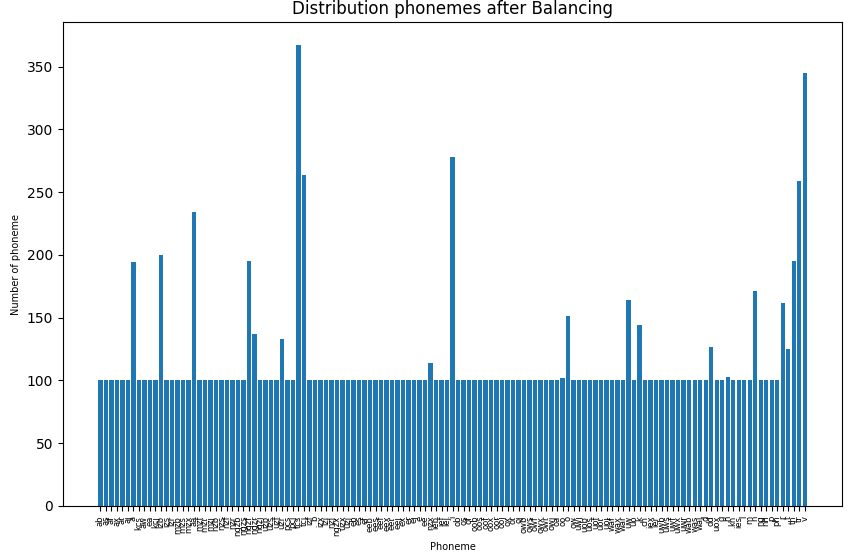
\includegraphics[scale=0.31]{charts/distribution_after.jpg}}
			\caption{Phân bố 134 âm vị tiếng Việt trong bộ dữ liệu sau khi được cân bằng}
			\label{fig_distribution_after}
		\end{figure}
	\end{frame}
	
	\begin{frame}{Trích xuất đặc trưng} \pause
		\begin{itemize}
			\item Sử dụng phương pháp trích xuất đặc trưng MFCCs (Mel Frequency Cepstral Coefficients).  \pause
			\begin{itemize}
				\item Mỗi frame có độ dài là 25ms, khoảng cách giữa 2 frame liên tiếp là 10ms. \pause
			\end{itemize}
			
		\end{itemize}
		%\begin{figure}[htbp]
		%	\centerline{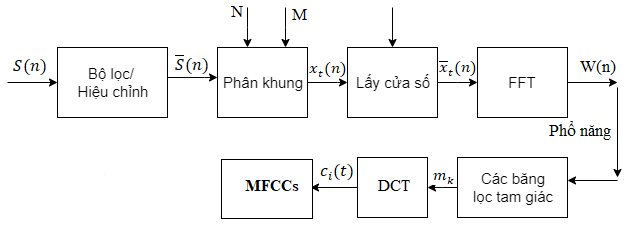
\includegraphics[scale=0.55]{charts/mfcc.png}}
		%	\caption[MFCCs]{Quá trình trích xuất đặc trưng MFCCs}
		%	\label{fig_mffc_extract}
		%\end{figure}
		\begin{columns}
			\begin{column}{0.5\textwidth}
				\begin{itemize}
					\item Mỗi frame trích xuất được một vector đặc trưng-13 chiều tương ứng. \pause
					\item "Rescale" lại đặc trưng thu được bằng Standardization:
					\[
					x^{'} = \frac{x - \mu}{\sigma + \epsilon}
					\]   \pause
					\begin{itemize}
						\item $\mu$ và $\sigma$ được tính dựa trên K (K=200) mẫu trong tập dữ liệu huấn luyện,
						\item $\epsilon$ = $1e-14$
					\end{itemize} \pause
				\end{itemize}
			\end{column}
			\begin{column}{0.5\textwidth}
				\begin{figure}[htbp]
					\centerline{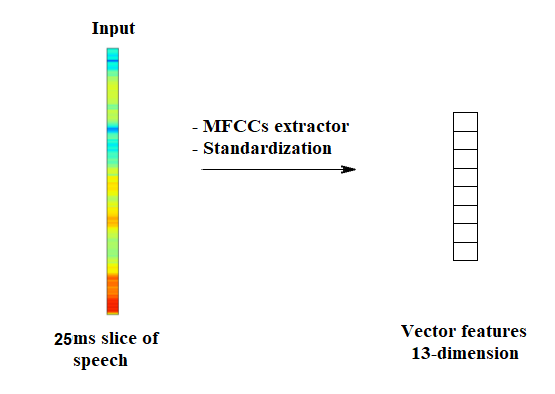
\includegraphics[scale=0.45]{charts/features_extract.png}}
					%\caption{Trích xuất đặc trưng cho một frame}
					\label{fig_frame_extract}
				\end{figure}
			\end{column}
		\end{columns}
		%\begin{itemize}
		%	\item "Rescale" lại đặc trưng thu được bằng Standardization:
		%	\[
		%	\]
		%\end{itemize}	
	\end{frame}
	
	\begin{frame}{Mô hình âm học}  \pause
		\begin{itemize}
			\item Mỗi vector đặc trưng thu được sau đó đưa qua mô hình âm học. Đầu ra của nó là một phân phối xác suất trên các class là bộ ký tự C.  \pause
			\item Bộ ký tự C bao gồm 89 chữ cái (gồm cả thanh điệu) trong Tiếng Việt, 1 ký tự \emph{"Space"}. Để tổng quát hơn, xét cả 4 ký tự trong tiếng Anh \emph{\{f, j, w, z\}} và ký tự \emph{"blank"} $\rightarrow$ Output = 95 units  \pause
			\begin{figure}[htbp]
				\centerline{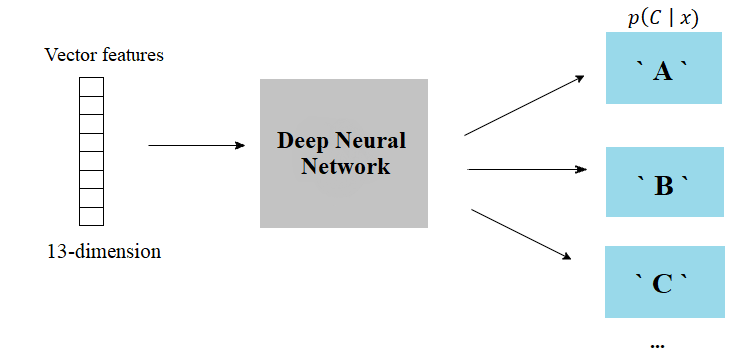
\includegraphics[scale=0.4]{charts/features2dnn.png}}
				%\caption{Trích xuất đặc trưng cho một frame}
				\label{fig_feature2dnn}
			\end{figure}  \pause
			\textbf{Input:} Một vector đặc trưng biểu diễn cho một frame của tín hiệu tiếng nói \\  \pause
			\textbf{Output:} Một phân phối xác suất trên bộ ký tự nhận dạng 
		\end{itemize}
	\end{frame}
	
	%\begin{frame}{Mô hình âm học}
	%	\begin{figure}[htbp]
	%		\centerline{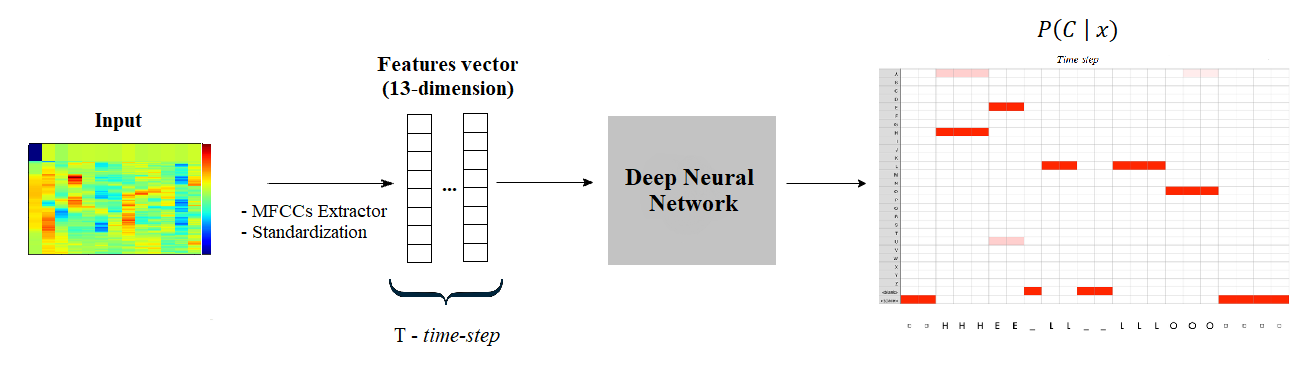
\includegraphics[scale=0.35]{charts/architecture_2.png}}
	%		%\caption[Overview architecture]{Tổng quan kiến trúc mô hình âm học được áp dụng.}
	%		\label{fig_architecture_overview}
	%	\end{figure}
	%\end{frame}
	
	\begin{frame}{Mô hình âm học}  \pause
		\begin{figure}[htbp]
			\centerline{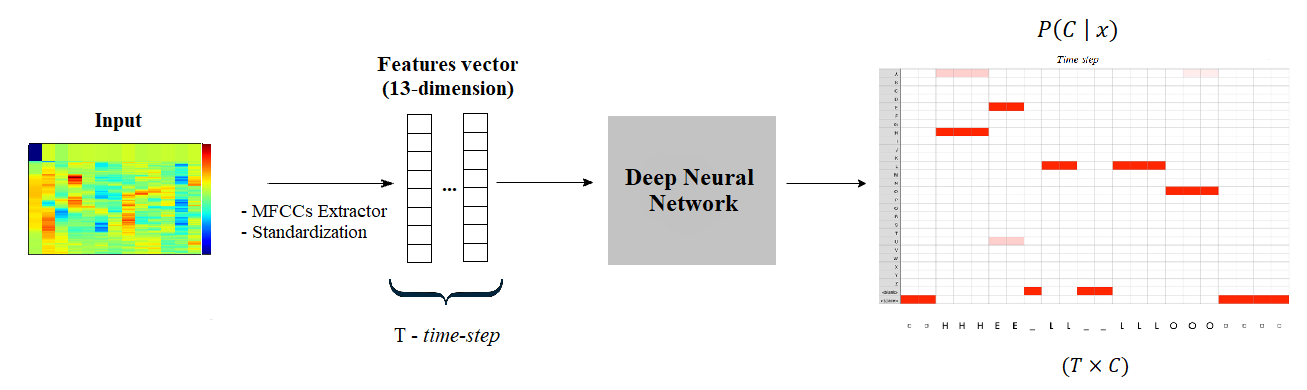
\includegraphics[scale=0.35]{charts/architecture_21.png}}
			%\caption[Overview architecture]{Tổng quan kiến trúc mô hình âm học được áp dụng.}
			\label{fig_architecture_overview}
		\end{figure}  \pause
		\textbf{Input:} Một tín hiệu tiếng nói (speech) được phát ra bởi người khuyết tật giọng nói \\  \pause
		\textbf{Output:} Một ma trận phân phối xác suất trên bộ ký tự C gồm 95 ký tự. 
	\end{frame}
	
	\begin{frame}{Mô hình âm học - Kiến trúc}  \pause
		\begin{itemize}
			\item Tham khảo kiến trúc mô hình của Deep Speech 1 \footnote{\text{\color{blue} Awni Hannun}, "Deep Speech: Scaling up end-to-end speech recognition". \emph{\color{blue} In: 	arXiv:1412.5567 (2014).}} và Deep Speech 2 \footnote{\text{\color{blue}Dario Amodei}, "Deep Speech 2: End-to-End Speech Recognition in English and Mandarin". \emph{\color{blue} In: arXiv:1512.02595 (2015).}}  \pause
			\begin{columns}
				\begin{column}{0.5\textwidth}
					\begin{itemize}
						\item Kiến trúc chung cho các thử nghiệm mô hình âm học 
					\end{itemize}
				\end{column}
				\begin{column}{0.5\textwidth}
					\begin{figure}[htbp]
						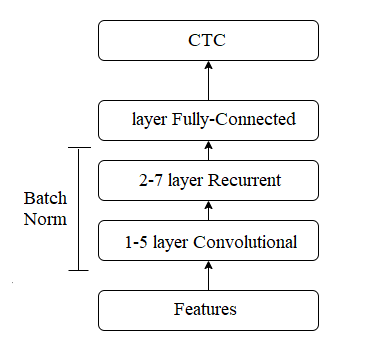
\includegraphics[scale=0.55]{charts/architecture.png}
						%\caption{Kiến trúc mô hình}
						\label{fig_architecture}
					\end{figure}
				\end{column}
			\end{columns}					
		\end{itemize}		
	\end{frame}
	
	\begin{frame}{Mô hình âm học - Kiến trúc}  \pause
		\begin{columns}
			\begin{column}{0.5\textwidth}
				\begin{figure}[htbp]
					\centerline{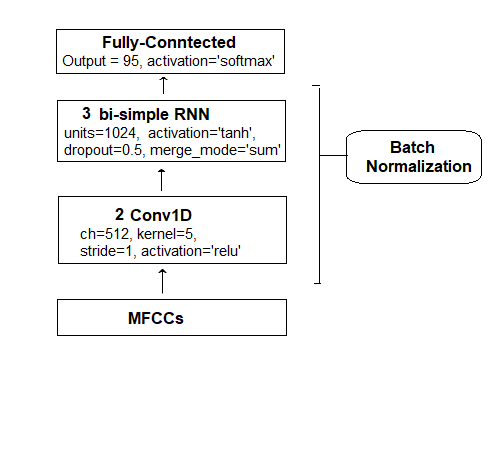
\includegraphics[scale=0.45]{charts/model1.png}}
					\caption{Model 1}
					\label{fig_model1}
				\end{figure}  \pause
			\end{column}
			\begin{column}{0.5\textwidth}
				\begin{figure}[htbp]
					\centerline{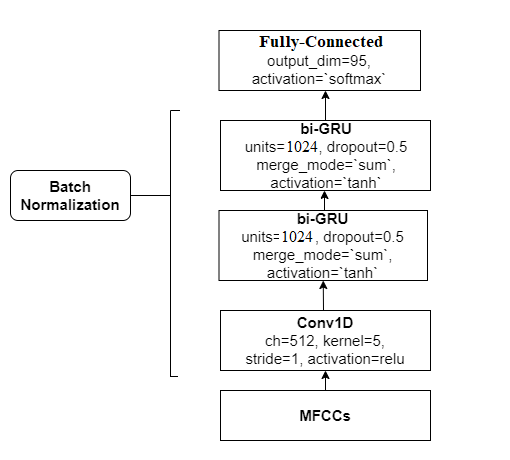
\includegraphics[scale=0.45]{charts/model2.png}}
					\caption{Model 2}
					\label{fig_model2}
				\end{figure}
			\end{column}
		\end{columns}
	\end{frame}
	
	\begin{frame}{Mô hình âm học}  \pause
		\begin{itemize}
			\item Training với hàm CTC loss (Connectionist Temporal Classification) \footnote{\text{\color{blue} Alex Graves}, "Towards End-to-End Speech Recognition with Recurrent Neural Networks". \emph{\color{blue} In ICML, 2014.}} \newline  \pause
			\item Sử dụng phương pháp tối ưu SGD (Stochastic Gradient Descent) với:  \pause
			\begin{itemize}
				\item learning rate = 0.01
				\item momentum = 0.9
				\item nesterov = True
				\item L2 weight decay = 1e-6
				\item clipnorm = 5				
			\end{itemize}
		\end{itemize}
	\end{frame}
	
	\begin{frame}{Decoding} \pause
		\begin{itemize}
			\item Để lấy được văn bản đầu ra cho tín hiệu tiếng nói đó, chúng ta cần phải thực hiện decoding (giải mã) ma trận output của mô hình âm học. \newline \pause
			\item Giải thuật để decoding: \newline \pause
			\begin{itemize}
				\item Greedy Search (Max decoding) \newline  \pause%\footnote{\text{\color{blue} Phan Xuân Phúc}"Thử nghiệm nhận dạng tiếng nói tiếng Việt cho người khuyết tật giọng nói". \emph{\color{blue}In ĐATN Đại học BHKN, 20191.}}
				%\begin{itemize}
					%\item Ở mỗi time-step (tức là, mỗi frame), ta lấy các ký tự có xác suất lớn nhất.
					%\item Sau đó, loại bỏ những ký tự lặp lại.
				%\end{itemize} 
				\item Beam Search \newline  \pause%\footnote{\text{\color{blue} Phan Xuân Phúc}"Thử nghiệm nhận dạng tiếng nói tiếng Việt cho người khuyết tật giọng nói". \emph{\color{blue}In ĐATN Đại học BHKN, 20191.}}
			\end{itemize} 
			\textbf{Input:} Một ma trận phân phối xác suất trên các ký tự \\  \pause
			\textbf{Output:} Một văn bản (text) đầu ra được giải mã (decoded output).
		\end{itemize}		
	\end{frame}
	
	\section{Kết quả đánh giá}
	\begin{frame}{Đánh giá mô hình}
		\begin{itemize}
			\item Mô hình được đánh giá dựa trên ba độ đo (metrics): \newline \pause
			\begin{itemize}
				\item CER (Char Error Rate): \emph{Tỷ lệ lỗi của ký tự}, \newline \pause
				\item WER (Word Error Rate): \emph{Tỷ lệ lỗi của từ}, \newline \pause
				\item SER (Sentence Error Rate): \emph{Tỷ lệ lỗi của câu}.\newline
			\end{itemize}
		\end{itemize}
	\end{frame}
	
	%\begin{frame}{Results}
	%	\begin{itemize}
	%		\item Kết quả thay đổi của hàm loss CTC sau 80 epochs của 2 mô hình:			
	%	\end{itemize}
	%		\centerline{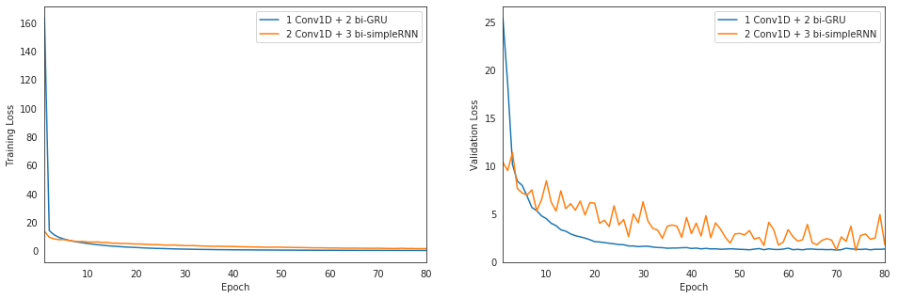
\includegraphics[scale=0.5]{charts/loss.png}}
	%		\caption{Kết quả thay đổi hàm loss CTC trong quá trình huấn luyện của 2 mô hình sau 80 epochs. Đường màu cam biểu thị cho \emph{Model 1} và đường màu xanh biểu thị cho \emph{Model 2}.}
	%		\label{fig_loss}
	%	\end{figure}
	%\end{frame}
	
	\begin{frame}{Kết quả}		
		\begin{table}
			\begin{center}
				\resizebox{\linewidth}{!}{
					\tiny
					\begin{tabular}{l  c  c  c}
						& CER & WER & SER\\
						\hline \hline
						& & &\\
						Model 1 & 17.03 & 41.70 & 42.44\\
						& & &\\
						Model 2 & \text{\color{red}7.73} & \text{\color{red}19.67} & \text{\color{red}20.16}\\
						& & &\\
						\hline
				\end{tabular}}
				\caption{So sánh kết quả hai mô hình dựa trên các độ đo CER, WER và SER (\%).}
			\end{center}
		\end{table} 
		\begin{itemize}
			\item Nhận xét:  \pause
			\begin{itemize}
				\item Mô hình sử dụng mạng GRU 2 chiều mang lại hiệu suất vượt trội so với mạng RNN thuần 2 chiều.
			\end{itemize}
		\end{itemize}
	\end{frame}
	
	\begin{frame}{Kết quả}
		\begin{table}
			\begin{center}
				\resizebox{\linewidth}{!}{
					\tiny
					\begin{tabular}{l  c  c  c}
						& CER & WER & SER\\
						\hline \hline
						& & &\\
						Google API & 75.34 & 90.21 & 91.51\\
						& & &\\
						\hline
				\end{tabular}}
				\caption{Kết quả đánh giá khi sử dụng Google API nhận dạng tiếng nói Tiếng Việt của người khuyết tật giọng nói dựa trên các độ đo CER, WER và SER (\%).}
			\end{center}
		\end{table}
	\end{frame}
	
	\begin{frame}{Kết quả}
		\begin{figure}[htbp]
			\centerline{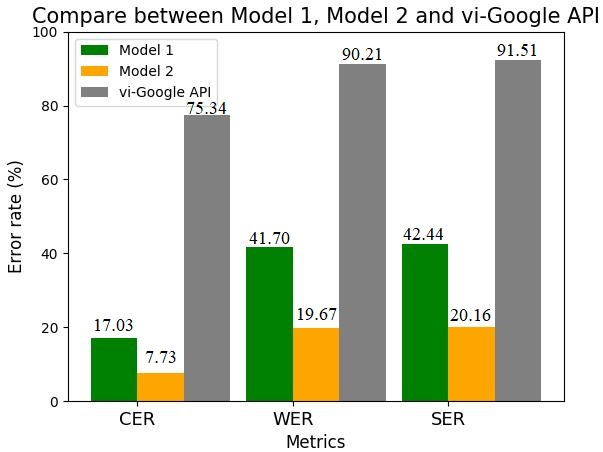
\includegraphics[scale=0.35]{charts/compare.jpg}}
			\caption{So sánh giữa các mô hình Model 1, Model 2 và sử dụng Google API}
			\label{fig_cp_model2_ggapi}
		\end{figure}
	\end{frame}
	
	\begin{frame}{Kết quả}
		\begin{figure}[htbp]
			\centerline{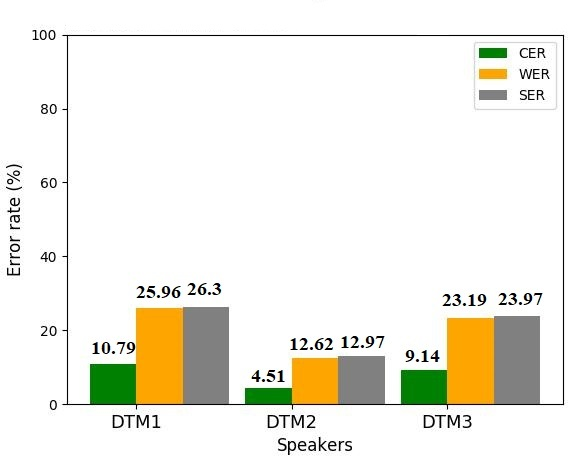
\includegraphics[scale=0.35]{charts/model2_everyone.jpg}}
			\caption{Kết quả đánh giá của Model 2 cho từng người nói \emph{(DTM1, DTM2, DTM3)}}
			\label{fig_cp_model2_everyone}
		\end{figure}
	\end{frame}
	
	\begin{frame}{Nhận xét tổng quan} \pause
		\begin{alertblock}{Nhận xét một số trường hợp dẫn đến nhận dạng sai dựa trên phân tích định tính đầu ra:}  \pause
			\begin{itemize}
				\item Các chữ cái phát âm giống nhau, ví dụ như: "ia" với "ya"; "iê" với "yê"; "i" với "y"; "âu" với "ô"; "au" với "o"; ...  \pause
				\item Một số chữ cái mà người khuyết tật khó phát âm phân biệt, nhận dạng bị lệch lạc như: "tr" với "t"; "x" với "s"; "gi" với "d"; "nh" với "n"; "kh" với "c"; ...  \pause
				\item Một số trường hợp nhận diện bị thiếu âm, chẳng hạn như "trong" thành "tong" hoặc "rong"; "dấu" thành "ấu"; ... \pause
				\item Ngoài ra mô hình vẫn còn nhận dạng sai khi xuất hiện nhiễu phát âm hoặc môi trường. \pause
			\end{itemize}
		\end{alertblock}
	\end{frame}

	\section{Kết luận và hướng phát triển trong tương lai}
	\begin{frame}{Kết luận}
		\begin{block}{Kết quả đạt được}  \pause
			\begin{itemize}
				\item Thực hiện quá trình thu thập và xử lý dữ liệu  \pause
				\item Tìm hiểu, nghiên cứu xử lý tiếng nói và trích xuất đặc trưng cho âm thanh tiếng nói  \pause
				\item Nghiên cứu các mô hình học âm học và thực hiện xây dựng mô hình giải quyết bài toán.  \pause
				\item Đánh giá, so sánh các mô hình và sử dụng Google API với nhau.
			\end{itemize}
		\end{block}
	\end{frame}
	
	\begin{frame}{Kết luận}
		\begin{alertblock}{Vấn đề hạn chế}  \pause
			\begin{itemize}
				\item Vấn đề thu thập dữ liệu còn nhiều hạn chế về độ đa dạng về thời lượng, từ vựng, số lượng người nói.  \pause
				\item Việc trích xuất đặc trưng và decoding vẫn còn có thể được cải thiện.  \pause
				\item Việc huấn luyện và đánh giá mô hình còn hạn chế về thời gian và máy huấn luyện $\rightarrow$ hạn chế trong việc thử nghiệm thay đổi các tham số trong mô hình và quá trình huấn luyện.
			\end{itemize}
		\end{alertblock}
	\end{frame}
	
	\begin{frame}{Hướng phát triển trong tương lai}
		\begin{block}{Hướng phát triển trong tương lai}  \pause
			\begin{itemize}
				\item Giải quyết vấn đề dữ liệu: tăng cường dữ liệu; có thể thử nghiệm sử dụng các mô hình sinh hiệu quả để tăng cường dữ liệu tổng quan hơn, ...  \pause
				\item Cải thiện chất lượng việc trích xuất đặc trưng cho tiếng nói, mô hình âm học và việc decoding.   \pause
				\item Giải quyết các vấn đề thách thức như nhiễu môi trường, tốc độ, ...  \pause
				\item Tìm hiểu, nghiên cứu hướng tiếp cận chuyển đổi giọng nói giữa người khuyết tật và người nói chuẩn (Voice Conversion).
			\end{itemize}
		\end{block}
	\end{frame}

	\begin{frame}
		\centering{\textbf{\fontsize{25pt}{30pt} \color{blue} Cảm ơn thầy cô và các bạn đã lắng nghe !}}
	\end{frame}

	\begin{frame}{Q \& A}
		\begin{center}
			\begin{figure}[htbp]
				\begin{center}
					
\includegraphics[width=0.75\linewidth]{charts/question-answer-problem.jpg}		
				\end{center}
				\label{fig_question_answer_problem}
			\end{figure}
		\end{center}
	\end{frame}

	
\end{document}
